\documentclass[../../dissertation.tex]{subfiles}
%\begin{Document}

\subsection{Grover}

%\begin{figure}[!h]
%	\centering
%	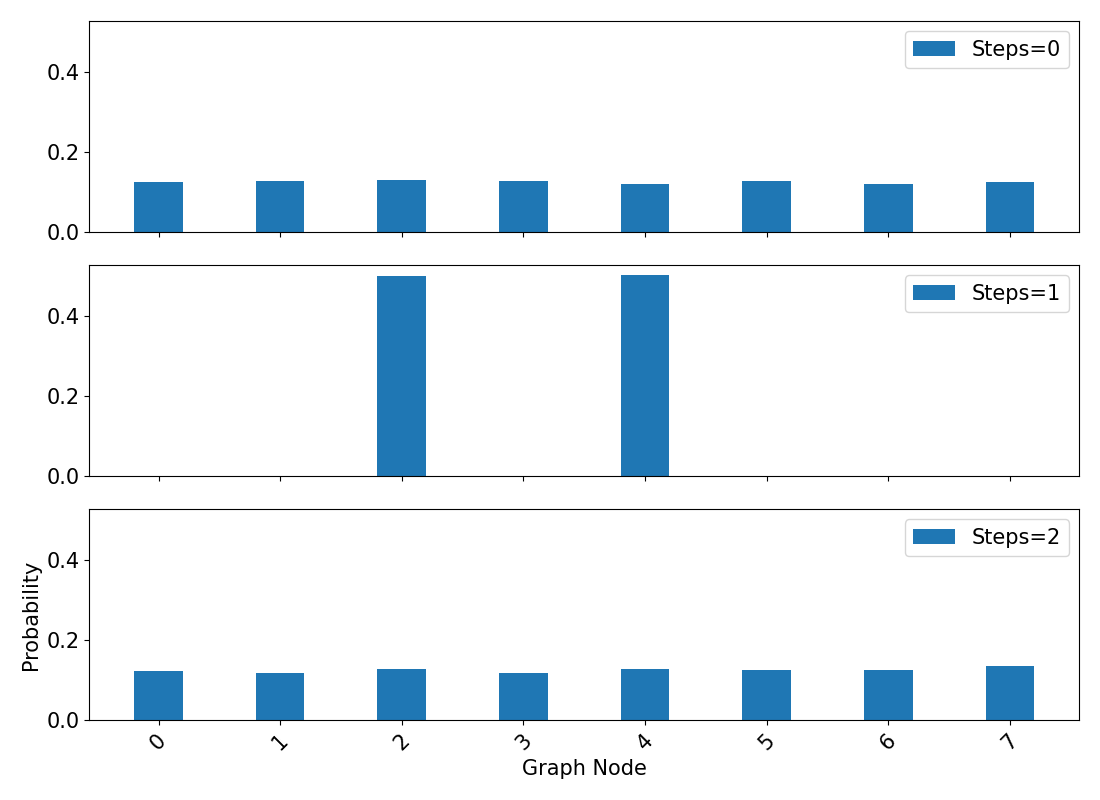
\includegraphics[scale=0.40]{img/Qiskit/GroverQiskit/GroverQiskitSearch_N3_M1_S012}
%	\caption{Probability distribution for the staggered quantum walk on a line after 50 steps, with initial condition $\ket{\Psi(0)}=\frac{\ket{0}+\ket{1}}{\sqrt{2}}$, for multiple angles.} 
%	\label{fig:fig5}
%\end{figure}
%
\subsection{Coined}
%
%\begin{figure}[!h]
%	\centering
%	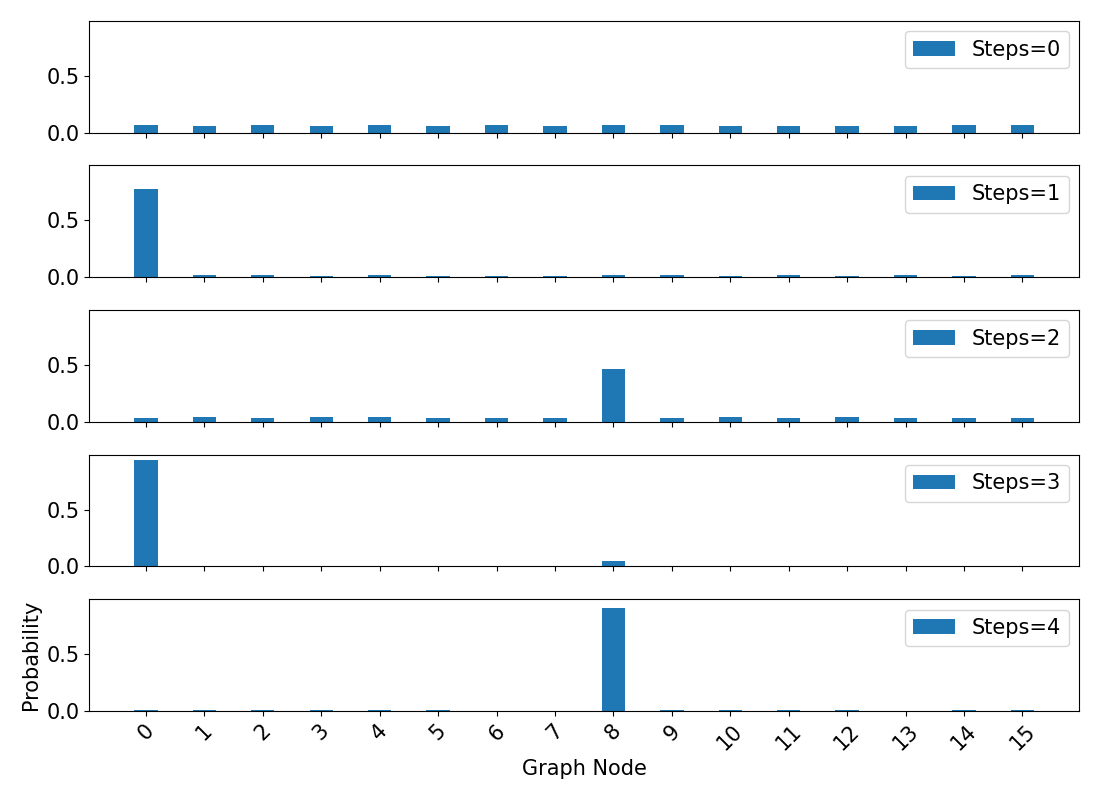
\includegraphics[scale=0.40]{img/Qiskit/CoinedQuantumWalk/Search/CoinedQiskitSearch_N4_M1_S01234}
%	\caption{Probability distribution for the staggered quantum walk on a line after 50 steps, with initial condition $\ket{\Psi(0)}=\frac{\ket{0}+\ket{1}}{\sqrt{2}}$, for multiple angles.} 
%	\label{fig:fig5}
%\end{figure}

%TODO: Fazer com outra moeda usando u3 com valores intermedios entre pi/2 ou pi/4
\subsection{Continuous}
\subsection{Staggered}

%\end{Document}
